\begin{frame}[allowframebreaks]{Denoising Autoencoders}
    \begin{itemize}
        \item \textbf{Corrupt input:} Introduce random noise to the input data, such as masking or adding Gaussian noise. The autoencoder is then trained to reconstruct the original, clean input from the corrupted version.
        \item \textbf{Robust feature learning:} By learning to recover the original data, the autoencoder is encouraged to extract meaningful and robust features that are less sensitive to noise and irrelevant variations.
        \item \textbf{Incremental understanding:} This approach helps the model generalize better by preventing it from simply memorizing the input, thus improving its ability to handle unseen or noisy data.
    \end{itemize}

    \framebreak

    \begin{figure}
        \centering
        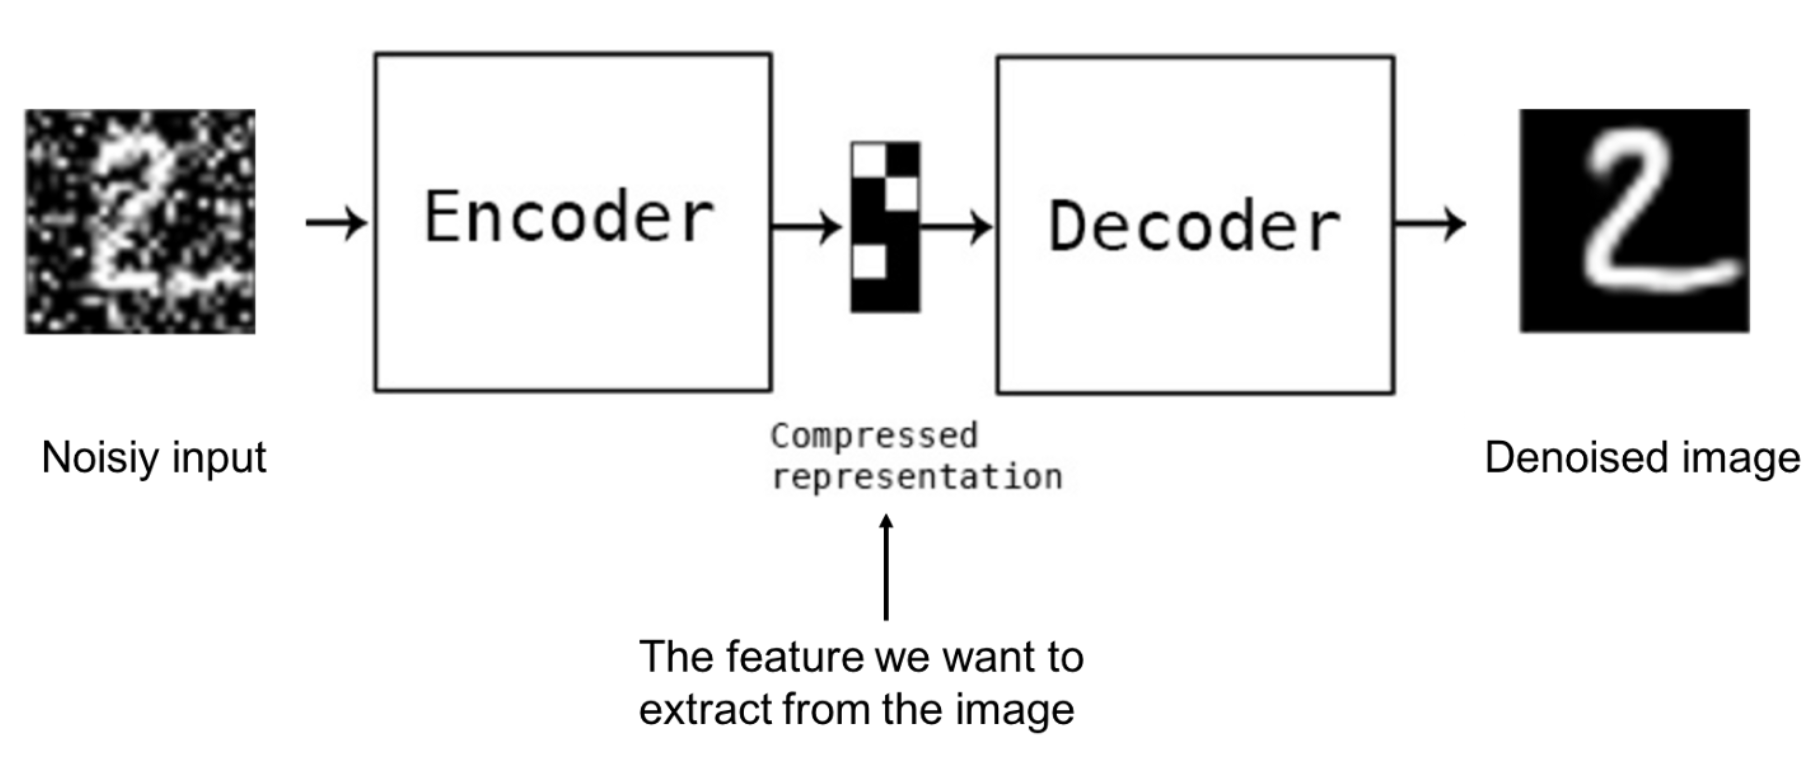
\includegraphics[width=\linewidth,height=0.9\textheight,keepaspectratio]{images/ssl/slide_12_1_img.png}
    \end{figure}

    \framebreak

    \begin{figure}
        \centering
        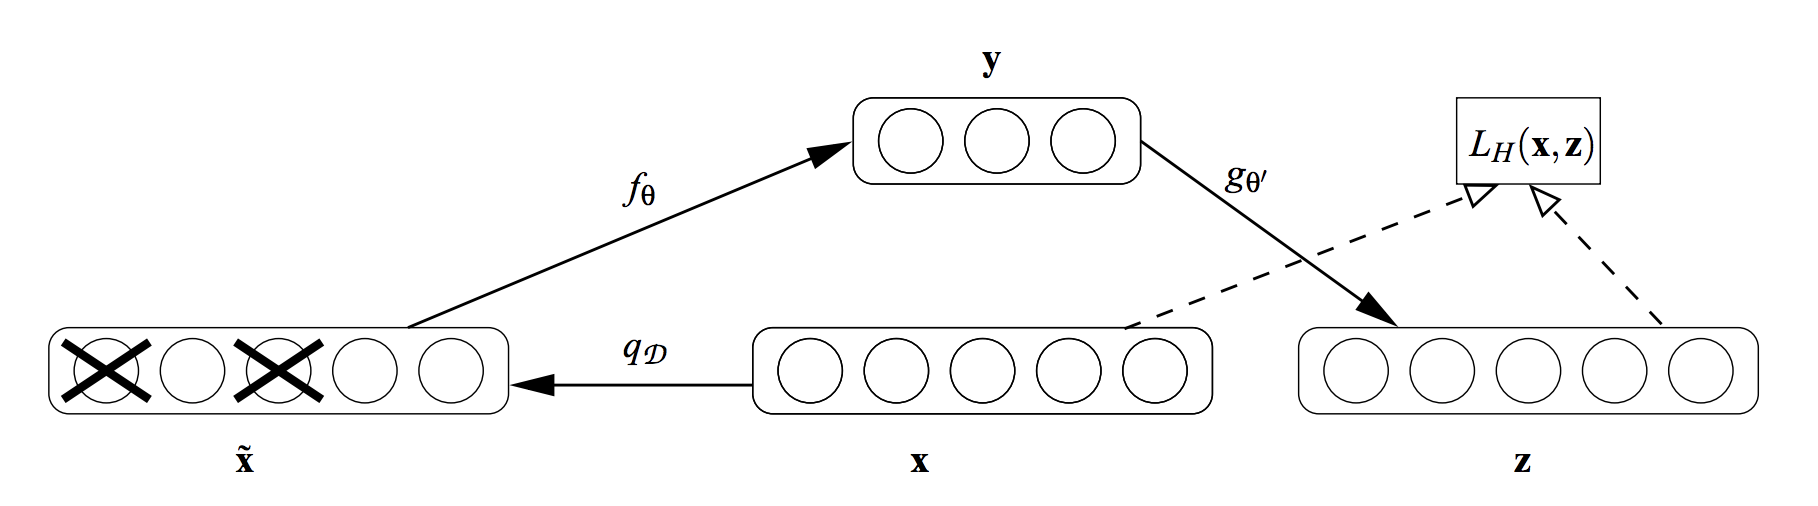
\includegraphics[width=\linewidth,height=0.9\textheight,keepaspectratio]{images/ssl/slide_13_1_img.png}
    \end{figure}

    \framebreak

    \begin{figure}
        \flushleft
        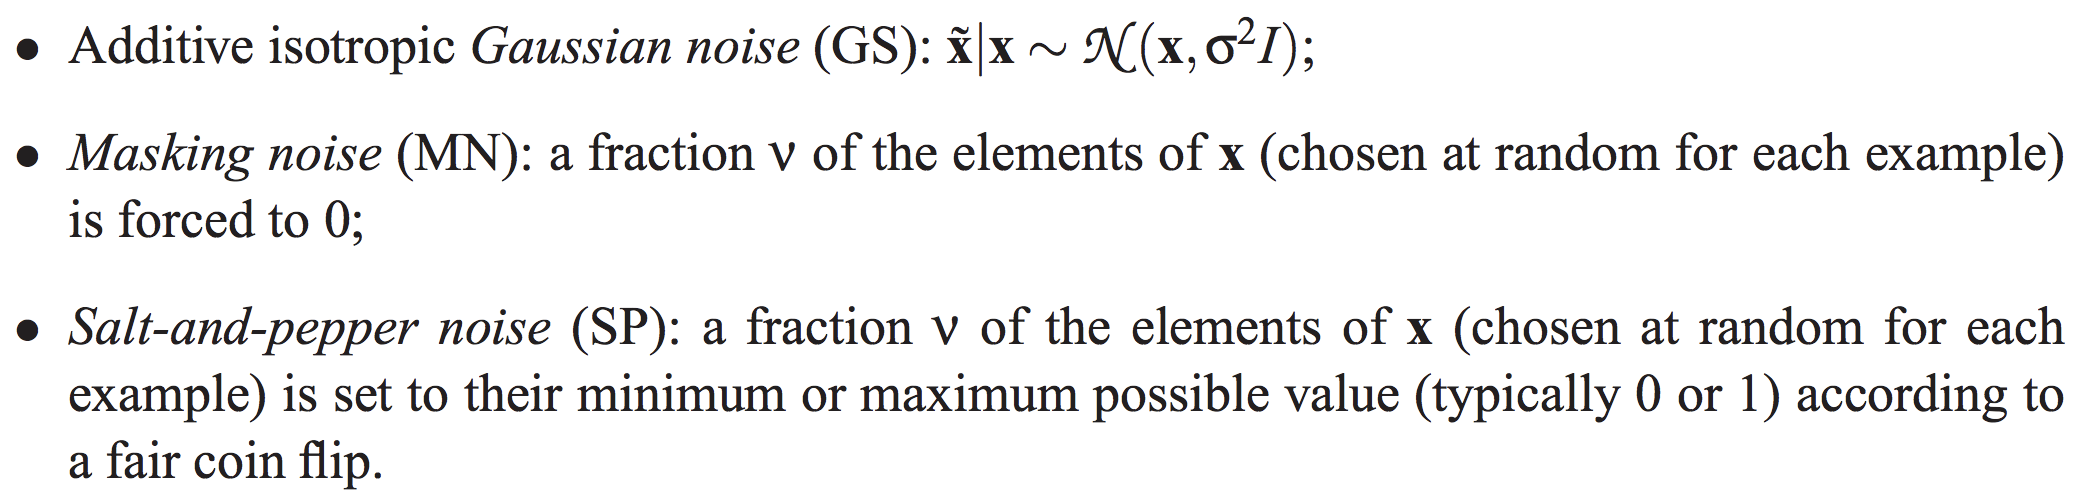
\includegraphics[width=1.08\linewidth,height=\textheight,keepaspectratio]{images/ssl/slide_14_1_img.png}
        \footnote{Vincent et al (2010). Denoising Autoencoders: Unsupervised Learning of Image Features from Noisy Data. ICML 2010.}
    \end{figure}
\end{frame}

\begin{frame}[allowframebreaks]{Emphasizing corrupted dimensions}
    \begin{figure}
        \flushleft
        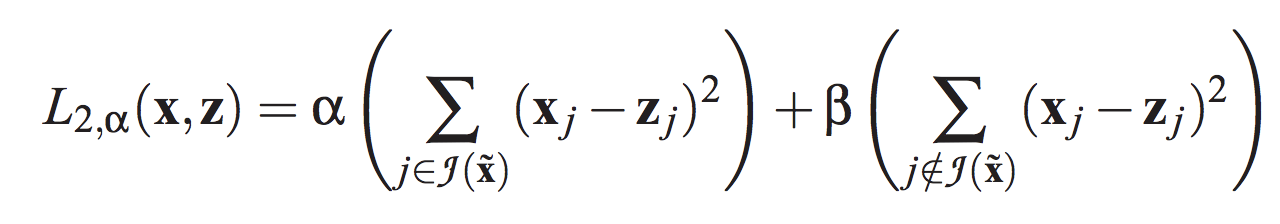
\includegraphics[width=1.08\linewidth,height=\textheight,keepaspectratio]{images/ssl/slide_15_1_img.png}
    \end{figure}

    \begin{figure}
        \flushleft
        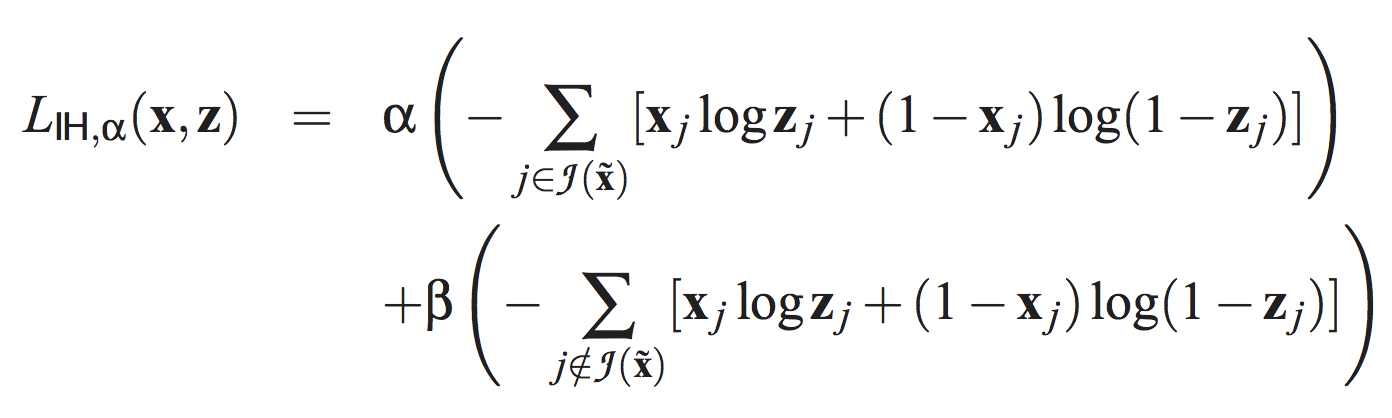
\includegraphics[width=1.08\linewidth,height=\textheight,keepaspectratio]{images/ssl/slide_15_2_img.png}
        \footnote{Vincent et al (2010). Denoising Autoencoders: Unsupervised Learning of Image Features from Noisy Data. ICML 2010.}
    \end{figure}
\end{frame}

\begin{frame}[allowframebreaks]{Denoising Autoencoders}
    \begin{figure}
        \flushleft
        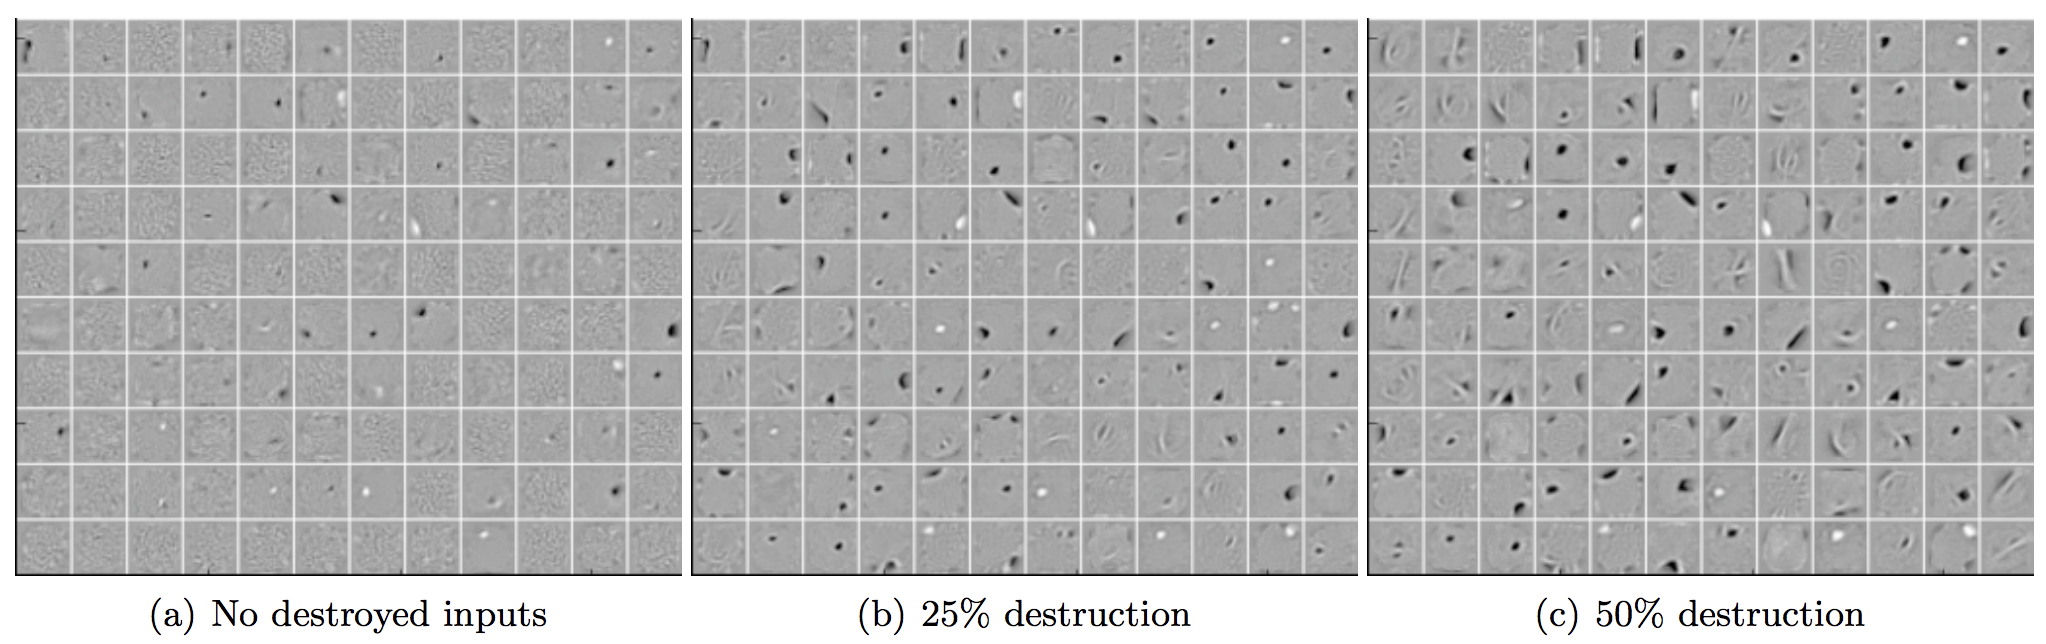
\includegraphics[width=1\linewidth,height=\textheight,keepaspectratio]{images/ssl/slide_16_1_img.png}
        \footnote{Vincent et al (2010). Denoising Autoencoders: Unsupervised Learning of Image Features from Noisy Data. ICML 2010.}
    \end{figure}
\end{frame}